% Draft for IEEE Access (formatted with IEEEtran journal; move to the IEEE Access template before submission).
% All numbers come from generated/numbers.tex (scripts/paper_numbers.py); do not type results by hand.
\documentclass[journal]{IEEEtran}
\usepackage{amsmath,amssymb}
\usepackage{graphicx}
\usepackage{booktabs}
\usepackage{array}
\usepackage{cite}
\usepackage{url}
\usepackage{xurl}            % long URLs may break anywhere
\usepackage{tikz}
\usetikzlibrary{arrows.meta,positioning,fit}
\setlength{\emergencystretch}{1em}  % room for long unbreakable intervals such as +0.135 [+0.115, +0.156]
\raggedbottom                % draft only: IEEE sets the final layout
\usepackage[hidelinks]{hyperref}
% Generated by scripts/paper_numbers.py from results/; do not edit by hand.
\newcommand{\BennuPSentry}{0.19}
\newcommand{\BrierPhaStratifiedAllFull}{0.0237}
\newcommand{\BrierPhaStratifiedAllStatic}{0.0255}
\newcommand{\BrierPhaStratifiedShortFull}{0.0056}
\newcommand{\BrierPhaStratifiedShortStatic}{0.0059}
\newcommand{\BrierPhaTemporalAllFull}{0.0102}
\newcommand{\BrierPhaTemporalAllStatic}{0.0105}
\newcommand{\BrierPhaTemporalShortFull}{0.0038}
\newcommand{\BrierPhaTemporalShortStatic}{0.0041}
\newcommand{\BrierSentryStratifiedAllFull}{0.0307}
\newcommand{\BrierSentryStratifiedAllStatic}{0.0361}
\newcommand{\BrierSentryStratifiedShortFull}{0.0495}
\newcommand{\BrierSentryStratifiedShortStatic}{0.0579}
\newcommand{\BrierSentryTemporalAllFull}{0.0422}
\newcommand{\BrierSentryTemporalAllStatic}{0.0480}
\newcommand{\BrierSentryTemporalShortFull}{0.0509}
\newcommand{\BrierSentryTemporalShortStatic}{0.0577}
\newcommand{\CostPhaStratifiedAllFull}{233}
\newcommand{\CostPhaStratifiedAllStatic}{245}
\newcommand{\CostPhaStratifiedShortFull}{147}
\newcommand{\CostPhaStratifiedShortStatic}{144}
\newcommand{\CostPhaTemporalAllFull}{159}
\newcommand{\CostPhaTemporalAllStatic}{166}
\newcommand{\CostPhaTemporalShortFull}{106}
\newcommand{\CostPhaTemporalShortStatic}{102}
\newcommand{\CostSentryStratifiedAllFull}{349}
\newcommand{\CostSentryStratifiedAllStatic}{429}
\newcommand{\CostSentryStratifiedShortFull}{529}
\newcommand{\CostSentryStratifiedShortStatic}{645}
\newcommand{\CostSentryTemporalAllFull}{493}
\newcommand{\CostSentryTemporalAllStatic}{596}
\newcommand{\CostSentryTemporalShortFull}{540}
\newcommand{\CostSentryTemporalShortStatic}{643}
\newcommand{\DPhaStratifiedAllDyn}{+0.013 [$-$0.000, +0.026]}
\newcommand{\DPhaStratifiedAllEns}{+0.029 [+0.014, +0.044]}
\newcommand{\DPhaStratifiedAllFocal}{+0.032 [+0.020, +0.046]}
\newcommand{\DPhaStratifiedAllFull}{+0.032 [+0.019, +0.046]}
\newcommand{\DPhaStratifiedShortDyn}{$-$0.019 [$-$0.054, +0.017]}
\newcommand{\DPhaStratifiedShortEns}{+0.073 [+0.019, +0.126]}
\newcommand{\DPhaStratifiedShortFocal}{+0.073 [+0.019, +0.129]}
\newcommand{\DPhaStratifiedShortFull}{+0.091 [+0.042, +0.147]}
\newcommand{\DPhaTemporalAllDyn}{$-$0.036 [$-$0.057, $-$0.010]}
\newcommand{\DPhaTemporalAllEns}{+0.002 [$-$0.029, +0.041]}
\newcommand{\DPhaTemporalAllFocal}{+0.012 [$-$0.019, +0.043]}
\newcommand{\DPhaTemporalAllFull}{+0.020 [$-$0.008, +0.052]}
\newcommand{\DPhaTemporalShortDyn}{+0.021 [$-$0.030, +0.058]}
\newcommand{\DPhaTemporalShortEns}{+0.068 [+0.003, +0.135]}
\newcommand{\DPhaTemporalShortFocal}{+0.112 [+0.049, +0.190]}
\newcommand{\DPhaTemporalShortFull}{+0.121 [+0.067, +0.194]}
\newcommand{\DSentryStratifiedAllDyn}{+0.039 [+0.024, +0.055]}
\newcommand{\DSentryStratifiedAllEns}{+0.133 [+0.113, +0.155]}
\newcommand{\DSentryStratifiedAllFocal}{+0.131 [+0.111, +0.151]}
\newcommand{\DSentryStratifiedAllFull}{+0.135 [+0.115, +0.156]}
\newcommand{\DSentryStratifiedShortDyn}{+0.034 [+0.019, +0.048]}
\newcommand{\DSentryStratifiedShortEns}{+0.132 [+0.110, +0.155]}
\newcommand{\DSentryStratifiedShortFocal}{+0.130 [+0.109, +0.151]}
\newcommand{\DSentryStratifiedShortFull}{+0.133 [+0.112, +0.155]}
\newcommand{\DSentryTemporalAllDyn}{+0.024 [+0.006, +0.041]}
\newcommand{\DSentryTemporalAllEns}{+0.127 [+0.104, +0.146]}
\newcommand{\DSentryTemporalAllFocal}{+0.125 [+0.103, +0.144]}
\newcommand{\DSentryTemporalAllFull}{+0.119 [+0.098, +0.139]}
\newcommand{\DSentryTemporalShortDyn}{+0.015 [$-$0.004, +0.031]}
\newcommand{\DSentryTemporalShortEns}{+0.124 [+0.099, +0.142]}
\newcommand{\DSentryTemporalShortFocal}{+0.122 [+0.098, +0.141]}
\newcommand{\DSentryTemporalShortFull}{+0.117 [+0.094, +0.134]}
\newcommand{\DynUncShareTopFifteen}{51}
\newcommand{\EnergyErr}{3.8\times10^{-10}}
\newcommand{\FlybyMaxErrKm}{42}
\newcommand{\FollowSenTempFull}{8.2}
\newcommand{\FollowSenTempStatic}{17.0}
\newcommand{\FracDminGeMoid}{98}
\newcommand{\FracUnbound}{0.08}
\newcommand{\MaxRankCorr}{0.984}
\newcommand{\NCalPosPhaTemp}{99}
\newcommand{\NDiam}{1,247}
\newcommand{\NDminLtFive}{10,738}
\newcommand{\NFocalPlain}{2}
\newcommand{\NFullFeat}{91}
\newcommand{\NIAS}{93}
\newcommand{\NLost}{0}
\newcommand{\NObj}{43,160}
\newcommand{\NPHA}{2,552}
\newcommand{\NPhaDisagree}{49}
\newcommand{\NSentry}{2,256}
\newcommand{\NShortArc}{24,592}
\newcommand{\NSigEns}{0}
\newcommand{\NSigFocal}{0}
\newcommand{\NSigMLP}{8}
\newcommand{\NSigUncOverDyn}{8}
\newcommand{\NStaticFeat}{41}
\newcommand{\NTorinoRated}{2,254}
\newcommand{\OOFPhaFull}{0.783}
\newcommand{\OOFPhaNaive}{0.999}
\newcommand{\OOFPhaStatic}{0.748}
\newcommand{\OOFSentryFull}{0.587}
\newcommand{\OOFSentryNaive}{0.635}
\newcommand{\OOFSentryStatic}{0.447}
\newcommand{\PRPhaStratifiedAllFull}{0.790}
\newcommand{\PRPhaStratifiedAllNaive}{0.999}
\newcommand{\PRPhaStratifiedAllStatic}{0.758}
\newcommand{\PRPhaStratifiedShortFull}{0.346}
\newcommand{\PRPhaStratifiedShortNaive}{0.973}
\newcommand{\PRPhaStratifiedShortStatic}{0.255}
\newcommand{\PRPhaTemporalAllFull}{0.540}
\newcommand{\PRPhaTemporalAllNaive}{0.998}
\newcommand{\PRPhaTemporalAllStatic}{0.520}
\newcommand{\PRPhaTemporalShortFull}{0.310}
\newcommand{\PRPhaTemporalShortNaive}{0.991}
\newcommand{\PRPhaTemporalShortStatic}{0.188}
\newcommand{\PRSentryStratifiedAllFull}{0.603}
\newcommand{\PRSentryStratifiedAllNaive}{0.655}
\newcommand{\PRSentryStratifiedAllStatic}{0.468}
\newcommand{\PRSentryStratifiedShortFull}{0.597}
\newcommand{\PRSentryStratifiedShortNaive}{0.657}
\newcommand{\PRSentryStratifiedShortStatic}{0.464}
\newcommand{\PRSentryTemporalAllFull}{0.533}
\newcommand{\PRSentryTemporalAllNaive}{0.583}
\newcommand{\PRSentryTemporalAllStatic}{0.415}
\newcommand{\PRSentryTemporalShortFull}{0.531}
\newcommand{\PRSentryTemporalShortNaive}{0.584}
\newcommand{\PRSentryTemporalShortStatic}{0.415}
\newcommand{\PalermoMax}{$-$0.98}
\newcommand{\PalermoMaxName}{29075 (1950 DA)}
\newcommand{\PctShortArc}{57}
\newcommand{\PrevPHA}{5.9}
\newcommand{\PrevSentry}{5.2}
\newcommand{\PriorDeltaPha}{$-$0.001}
\newcommand{\PriorDeltaSentry}{+0.002}
\newcommand{\ProbeHAll}{0.91}
\newcommand{\ProbeHDyn}{0.68}
\newcommand{\ProbeHObs}{0.85}
\newcommand{\ProbeHUnc}{0.92}
\newcommand{\ProbeHXDyn}{0.91}
\newcommand{\ProbeMoidAll}{0.82}
\newcommand{\ProbeMoidDyn}{0.53}
\newcommand{\ProbeMoidOrbit}{0.79}
\newcommand{\ProbeMoidUnc}{0.85}
\newcommand{\ProbeMoidXDyn}{0.81}
\newcommand{\RecPhaStratifiedAllFull}{59.3}
\newcommand{\RecPhaStratifiedAllStatic}{55.6}
\newcommand{\RecPhaStratifiedShortFull}{52.0}
\newcommand{\RecPhaStratifiedShortStatic}{39.2}
\newcommand{\RecPhaTemporalAllFull}{61.8}
\newcommand{\RecPhaTemporalAllStatic}{55.9}
\newcommand{\RecPhaTemporalShortFull}{56.7}
\newcommand{\RecPhaTemporalShortStatic}{40.5}
\newcommand{\RecSentryStratifiedAllFull}{39.3}
\newcommand{\RecSentryStratifiedAllStatic}{27.4}
\newcommand{\RecSentryStratifiedShortFull}{30.5}
\newcommand{\RecSentryStratifiedShortStatic}{21.0}
\newcommand{\RecSentryTemporalAllFull}{27.3}
\newcommand{\RecSentryTemporalAllStatic}{21.2}
\newcommand{\RecSentryTemporalShortFull}{24.5}
\newcommand{\RecSentryTemporalShortStatic}{18.5}
\newcommand{\SnapshotDate}{2026-11-22}
\newcommand{\SpearmanDminMoid}{0.71}
\newcommand{\TopFeatSentry}{unc\_p\_dmin\_lt\_001}
\newcommand{\TopFeatSentryShare}{22.9}
\newcommand{\TorinoMax}{0}
\newcommand{\TrivCostSentryTemporal}{934}
\newcommand{\UncCoverage}{99.7}
\newcommand{\UncOverDynPhaTemporal}{+0.056 [+0.032, +0.082]}
\newcommand{\UncOverDynSentryTemporal}{+0.094 [+0.077, +0.115]}
\newcommand{\WallEvalMax}{26}
\newcommand{\WallEvalMin}{6}
\newcommand{\WallStageThree}{92}
\newcommand{\WallStageTwo}{4.6}


\begin{document}

\title{Leakage-Free, Uncertainty-Aware Classification of Near-Earth Asteroid Hazard with N-Body Dynamics and Covariance Clones}

\author{\IEEEauthorblockN{Author Name\IEEEauthorrefmark{1}}
\IEEEauthorblockA{\IEEEauthorrefmark{1}Department, Institution, City, Country}
\thanks{Corresponding author: Author Name (e-mail: author@institution.edu).}}

\maketitle

\begin{abstract}
Published machine-learning classifiers that label near-Earth asteroids as potentially hazardous (PHAs) often report accuracies above 94\%, yet many use the minimum orbit intersection distance (MOID) and absolute magnitude $H$ as inputs, the two quantities that define the PHA label. We quantify this circularity and build a classifier that never sees them. Using \NObj{} near-Earth objects from the JPL Small-Body Database with full orbit covariances, we target two labels: the PHA flag (Mode A, \PrevPHA\% positive) and membership of JPL's Sentry impact-monitoring list (Mode B, \PrevSentry\% positive). Name and rank-correlation gates block any input that reconstructs MOID or $H$, and a probe model measures how much of either remains implicitly recoverable. We add 50-year N-body propagation features and 32 covariance clones per object, propagated through the same dynamics, and evaluate LightGBM, an asymmetric focal loss, a dual-branch network and an ensemble on stratified and discovery-time splits with five seeds and paired bootstrap intervals. With MOID and $H$ the PHA task is trivial (PR-AUC \PRPhaStratifiedAllNaive); without them the static baseline reaches \PRPhaStratifiedAllStatic. Dynamics and uncertainty features raise PR-AUC by \DSentryStratifiedAllFull{} (Sentry, stratified) and \DSentryTemporalAllFull{} (Sentry, temporal), and by \DPhaStratifiedAllFull{} for the PHA label, with the largest relative gains on short-arc objects. In direct paired tests, the clone features improve on dynamics alone in all \NSigUncOverDyn{} settings, while neither the focal loss nor the ensemble differs significantly from log-loss LightGBM in any setting. Label-conditional conformal prediction gives finite-sample coverage for follow-up decisions. We release code, out-of-fold scores, per-object explanations and an interactive atlas, and we state the limits of the study, including partial emulation of Sentry's own method.
\end{abstract}

\begin{IEEEkeywords}
Near-Earth objects, planetary defense, data leakage, gradient boosting, N-body simulation, uncertainty quantification, conformal prediction, explainable AI.
\end{IEEEkeywords}

\section{Introduction}
\IEEEPARstart{A}{steroid} impact hazard is assessed operationally by orbit determination followed by impact monitoring, in which each object's orbit uncertainty is propagated to search for virtual impactors \cite{milani2005,roa2021}; results are summarised on the Palermo and Torino scales \cite{chesley2002,binzel2000}. In parallel, a growing number of studies train machine-learning classifiers to label near-Earth objects as potentially hazardous \cite{malakouti2023,bora2024,jacques2025,delina2024}. The PHA designation is a deterministic rule,
\begin{equation}
\mathrm{PHA} \iff \mathrm{MOID}_{\oplus} \le 0.05~\mathrm{au} \;\wedge\; H \le 22,
\label{eq:pha}
\end{equation}
and several of these studies use MOID, $H$ or close-approach distances among the inputs, identify them as the most important features \cite{bora2024}, and report accuracies of 94--99\% \cite{malakouti2023,jacques2025}. A classifier given the defining quantities can reproduce the rule without learning anything about hazard. This is a case of target leakage \cite{kaufman2012}.

Three further gaps limit the usefulness of such classifiers. Most use a single static set of osculating elements, although close encounters change orbits over decades. Most ignore orbit-determination uncertainty, although an object with a short observation arc can have a nominal orbit far from its true one, which is the case impact monitoring exists to handle \cite{milani2005}. Finally, they address the strong class imbalance with resampling such as SMOTE \cite{chawla2002} and report accuracy, a metric that is uninformative at 5\% prevalence \cite{saito2015}.

We make five contributions.
\begin{enumerate}
\item A \emph{leakage-controlled protocol} for NEO hazard classification: MOID, $H$ and every input that reconstructs them are blocked by name and rank-correlation gates. A probe quantifies the information that remains implicitly recoverable from legitimate inputs ($R^2=\ProbeHAll$ for $H$, $\ProbeMoidAll$ for MOID).
\item \emph{Physics-informed features} from 50-year N-body propagation of all \NObj{} objects, and from 32 covariance clones per object propagated through the same dynamics.
\item A careful evaluation with two labels, stratified and discovery-time splits, five seeds, paired stratified bootstrap intervals, a short-arc stratum, an ablation, and direct paired tests between model variants.
\item A \emph{decision layer}: calibrated probabilities, a cost-optimal threshold and label-conditional (Mondrian) conformal sets with finite-sample coverage \cite{vovk2005,angelopoulos2023}.
\item An open release: code, out-of-fold scores, TreeSHAP explanations for every object \cite{lundberg2020}, and an interactive atlas. Positions in the atlas are validated against JPL Horizons \cite{jplhorizons}.
\end{enumerate}

The paper is organised as follows. Section~\ref{sec:related} reviews related work. Section~\ref{sec:data} describes the data, labels and leakage controls, and Section~\ref{sec:methods} the features, models and evaluation. Section~\ref{sec:results} reports results, Section~\ref{sec:discussion} discusses limitations and threats to validity, and Section~\ref{sec:availability} describes the release.

\section{Related Work}\label{sec:related}
\emph{Impact monitoring.} JPL's Sentry and its successor Sentry-II sample the orbit-uncertainty region and integrate it forward to find virtual impactors, including non-gravitational forces where needed \cite{roa2021}; earlier systems searched the line of variations, a one-dimensional parametrisation of the uncertainty region \cite{milani2005}. Impact probabilities are combined with energy and time to impact on the Palermo scale \cite{chesley2002}, and communicated to the public on the Torino scale \cite{binzel2000}. These systems are the reference for risk: the present work does not replace them, but asks what a fast, transparent model learns from the same kinds of information, and whether it can help prioritise follow-up.

\emph{Machine learning for PHAs.} Prior classifiers use tree ensembles, neural networks and graph neural networks on catalogue features \cite{malakouti2023,bora2024,jacques2025,delina2024}. Malakouti et al.\ include the minimum orbit intersection, absolute magnitude and miss distances among the inputs \cite{malakouti2023}. Bora et al.\ combine machine learning with N-body integration and report MOID and $H$ as crucial features \cite{bora2024}. Jacques models asteroids as a similarity graph and applies SMOTE to a 0.22\%-prevalence label \cite{jacques2025}. We are not aware of prior work that removes the label-defining inputs, measures residual leakage, or uses covariance-based uncertainty as model input.

\emph{Population and physical properties.} Debiased population models describe the orbit and magnitude distribution of NEOs \cite{granvik2018}. Albedo and density depend on taxonomic complex \cite{thomas2011,carry2012}, and survey albedos are available for a subset of objects \cite{mainzer2011}. Thermal recoil (the Yarkovsky effect) changes semi-major axes over decades and matters for long-term impact predictions \cite{bottke2006}.

\emph{Imbalance, calibration and uncertainty in ML.} For rare positives, precision--recall analysis is more informative than ROC analysis \cite{davis2006,saito2015}. Alternatives to resampling include cost-sensitive objectives such as the focal loss \cite{lin2017} and threshold-moving on calibrated probabilities \cite{platt1999}. Conformal prediction provides distribution-free coverage guarantees, and its label-conditional (Mondrian) form controls the miss rate separately for each class \cite{vovk2005,angelopoulos2023}. Data leakage, including target leakage through features that encode the label, is a known source of inflated results \cite{kaufman2012}.

\section{Data, Labels and Leakage Controls}\label{sec:data}
\subsection{Data}
We downloaded all near-Earth objects with a numerical orbit solution and covariance from the JPL Small-Body Database, together with the Sentry list, on \SnapshotDate{} \cite{jplsbdb}. This gives \NObj{} objects. For each object we use its osculating elements and their formal uncertainties; observation metadata (data arc, number of observations, condition code, residual RMS, time since last observation); and physical information where measured (diameter for \NDiam{} objects, rotation period, taxonomy). Missing values are kept as missing, with explicit masks rather than mean imputation. Objects with a data arc shorter than 30~days form the \emph{short-arc stratum} (\NShortArc{} objects, \PctShortArc\%). Table~\ref{tab:features} lists the feature groups.

\begin{table}[t]
\caption{Input features. The first four groups form the leak-free static set (\NStaticFeat{} inputs).}
\label{tab:features}
\centering
\footnotesize
\begin{tabular}{>{\raggedright\arraybackslash}p{0.30\columnwidth}c>{\raggedright\arraybackslash}p{0.47\columnwidth}}
\toprule
Group & $n$ & Examples\\
\midrule
Orbital elements and derived & 12 & $a, e, i, q, Q$, angles as sin/cos, $T_J$\\
Observation metadata & 12 & data arc, $n_{\mathrm{obs}}$, radar, condition code, RMS, formal $\sigma$, staleness\\
Physical (measured, masked) & 6 & diameter, rotation period, taxonomy\\
Missingness masks & 11 & one indicator per field that can be missing\\
N-body dynamics & 19 & $\Delta a,\Delta e,\Delta i$ at 10/25/50 yr, $d_{\min}$, encounters, divergence\\
Covariance clones & 19 & clone $d_{\min}$ spread and quantiles, $P(d_{\min}<0.05,0.01$ au$)$, $\sigma$ of elements\\
Physical priors & 12 & albedo/density priors, $v_\infty$, impact speed, mass, energy\\
\midrule
Total (full model) & 91 & \\
\bottomrule
\end{tabular}

\end{table}

\subsection{Labels}
\emph{Mode A} is the PHA flag (\NPHA{} positives, \PrevPHA\%); the flag disagrees with rule~\eqref{eq:pha} recomputed from the catalogue for \NPhaDisagree{} objects, and we use the flag as published. \emph{Mode B} is membership of the Sentry list (\NSentry{} objects, \PrevSentry\%), which marks objects with at least one virtual impactor found by impact monitoring. In our snapshot, all \NTorinoRated{} Torino-rated Sentry objects are at level \TorinoMax{}, and the highest cumulative Palermo value is \PalermoMax{} (\PalermoMaxName). Mode B is therefore a list of ``objects whose impact probability is not yet ruled out'', not of likely impactors.

\subsection{Leakage controls}
Every model except the deliberately circular baseline passes two gates before training. A \emph{name gate} rejects features derived from MOID, $H$, the PHA flag or any Sentry output. A \emph{rank-correlation gate} rejects any feature $x_j$ whose Spearman correlation with an audit column $a_k$ (MOID, $H$, the flags, Sentry outputs) satisfies
\begin{equation}
\max_k \,\lvert \rho_s(x_j, a_k) \rvert > 0.995 ;
\end{equation}
the largest observed value over all accepted features is \MaxRankCorr. Diameter combined with albedo reconstructs $H$ through $D = 1329\,\mathrm{km}\cdot p_V^{-1/2}\,10^{-H/5}$, so albedo is kept out of the inputs.

The gates prevent direct access but not implicit recoverability. We therefore train a gradient-boosted regressor to predict $H$ and MOID from each group of legitimate inputs, with five-fold cross-validation (Table~\ref{tab:probe}). Orbital elements predict MOID well ($R^2=\ProbeMoidOrbit$), as expected, since MOID is a function of the orbit; observation metadata predict $H$ ($R^2=\ProbeHObs$), because faint objects are observed differently. Dynamics features alone recover less ($R^2=\ProbeHDyn$ for $H$, $\ProbeMoidDyn$ for MOID) and add nothing beyond the static inputs ($\ProbeHXDyn$ and $\ProbeMoidXDyn$ combined). These are physical relations, not leaks, but they bound what ``leak-free'' can mean: the models cannot read MOID or $H$, yet part of their information is present.

\begin{table}[t]
\caption{Residual information: cross-validated $R^2$ of a probe predicting $H$ and MOID from groups of leak-free inputs.}
\label{tab:probe}
\centering
\begin{tabular}{lcc}
\toprule
Input group & $R^2(H)$ & $R^2(\mathrm{MOID})$\\
\midrule
Orbital elements only & 0.57 & 0.79\\
Observation metadata only & 0.85 & 0.58\\
Physical (masked) only & 0.16 & 0.02\\
Orbit + observation & 0.91 & 0.82\\
All leak-free inputs & 0.91 & 0.82\\
All + uncertainty features & 0.92 & 0.85\\
\bottomrule
\end{tabular}

\end{table}

\section{Methods}\label{sec:methods}
Fig.~\ref{fig:pipeline} summarises the pipeline.

\begin{figure*}[t]
\centering
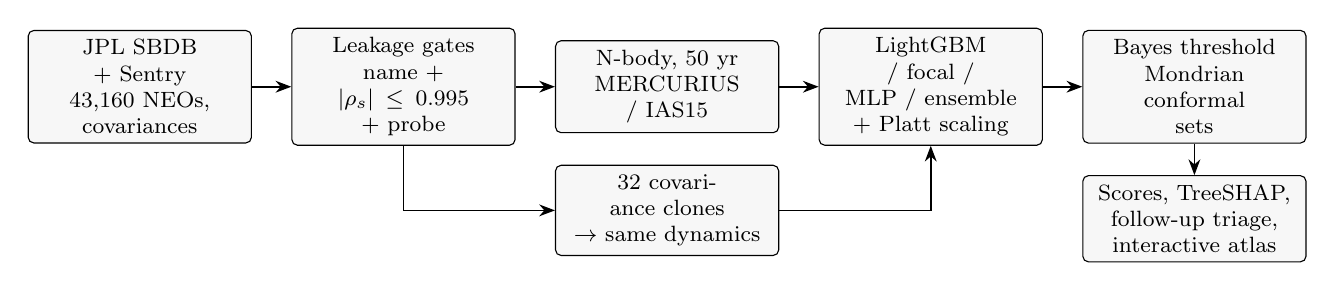
\begin{tikzpicture}[node distance=4mm and 5mm, font=\footnotesize,
  box/.style={draw, rounded corners=2pt, align=center, minimum height=10mm, text width=26mm, fill=black!3},
  arr/.style={-{Stealth[length=2mm]}, semithick}]
\node[box] (sbdb) {JPL SBDB + Sentry\\ \NObj{} NEOs,\\ covariances};
\node[box, right=of sbdb] (gate) {Leakage gates\\ name + $|\rho_s|\le0.995$\\ + probe};
\node[box, right=of gate] (nbody) {N-body, 50 yr\\ MERCURIUS / IAS15};
\node[box, below=of nbody] (clones) {32 covariance clones\\ $\to$ same dynamics};
\node[box, right=of nbody] (models) {LightGBM / focal /\\ MLP / ensemble\\ + Platt scaling};
\node[box, right=of models] (dec) {Bayes threshold\\ Mondrian conformal\\ sets};
\node[box, below=of dec] (out) {Scores, TreeSHAP,\\ follow-up triage,\\ interactive atlas};
\draw[arr] (sbdb) -- (gate); \draw[arr] (gate) -- (nbody); \draw[arr] (gate.south) |- (clones.west);
\draw[arr] (nbody) -- (models); \draw[arr] (clones.east) -| (models.south);
\draw[arr] (models) -- (dec); \draw[arr] (dec) -- (out);
\end{tikzpicture}
\caption{Pipeline. Static inputs pass the leakage gates; dynamics and clone features are computed from orbits and covariances only; models are calibrated and evaluated with a decision layer.}
\label{fig:pipeline}
\end{figure*}

\subsection{N-body dynamics}
All objects are propagated for 50 years from a common epoch with REBOUND \cite{rein2012}. We use the MERCURIUS hybrid integrator \cite{rein2019} with a 1-day step, switching to IAS15 \cite{rein2015} for the \NIAS{} objects whose perihelion passage would span fewer than three steps. The Sun, Venus, the Earth--Moon barycentre, Mars, Jupiter and Saturn are active bodies. Their initial conditions come from Standish's approximate elements \cite{standish}, with position errors of order $10^{-4}$~au for the inner planets; a DE440 ephemeris \cite{park2021} can be substituted. Objects whose orbit solutions refer to different epochs are first integrated to a common epoch.

Features include the changes $\Delta a$, $\Delta e$ and $\Delta i$ at 10, 25 and 50 years; the minimum Earth distance $d_{\min}$ over the window and its time; the number of encounters within 0.05~au; and the growth rate of the separation between each object and a shadow particle offset by its formal $1\sigma$ uncertainty, a Lyapunov-type proxy for chaos. The maximum relative energy error is $\EnergyErr$, no object is lost, and $d_{\min}\ge$ MOID for \FracDminGeMoid\% of objects, as expected, since MOID is a lower bound on the separation (Spearman $\rho=\SpearmanDminMoid$).

\subsection{Covariance clones}
For each object we draw $K=32$ samples of the cometary elements $\mathbf{x}=(e,q,t_p,\Omega,\omega,i)$ from $\mathcal{N}(\boldsymbol{\mu},\boldsymbol{\Sigma})$, using the full JPL covariance. Where non-gravitational parameters are estimated, the leading $6\times6$ block is used. To be robust to near-singular covariances, we factor the correlation matrix,
\begin{equation}
\boldsymbol{\Sigma} = \mathbf{D}\mathbf{R}\mathbf{D},\quad \mathbf{R}=\mathbf{V}\boldsymbol{\Lambda}\mathbf{V}^{\top},\quad
\mathbf{x}_{k,\pm} = \boldsymbol{\mu} \pm \mathbf{D}\mathbf{V}\boldsymbol{\Lambda}^{1/2}\mathbf{z}_k,
\end{equation}
with $\mathbf{z}_k\sim\mathcal{N}(\mathbf{0},\mathbf{I})$ for $k=1,\dots,K/2$, so the clone mean is exactly $\boldsymbol{\mu}$ (antithetic sampling). Clones are converted to Keplerian elements ($a=q/(1-e)$, $M=n(t-t_p)$), aligned to the common epoch, and re-centred on the N-body nominal state, so that the dispersion comes from the covariance while the centre matches the full-force orbit. They are then propagated with the same dynamics. Clones covered \UncCoverage\% of objects; unbound draws (\FracUnbound\% on average) are counted, not resampled. Features summarise each cloud, for example
\begin{equation}
\hat P(d_{\min}<\delta) = \frac{1}{K}\sum_{k=1}^{K} \mathbf{1}\!\left[d_{\min,k}<\delta\right]
\end{equation}
for $\delta\in\{0.05,0.01\}$~au, together with the spread and 5th percentile of $d_{\min,k}$, the spread of encounter times and of $\Delta a$ at 50 years, and covariance-shape statistics (formal $\sigma$ of each element, line-of-variations scale, condition number).

\subsection{Physical priors}
Albedo and bulk density priors are assigned by taxonomic complex, with explicit masks. S and C values follow Thomas et al.\ (NEO albedo; S 0.26, C 0.13) \cite{thomas2011} and Carry (density; S $2.72\pm0.54$, C $1.33\pm0.58$~g\,cm$^{-3}$) \cite{carry2012}. The X complex, the ``other'' class and the mixture used for objects without taxonomy are stated assumptions. The encounter speed follows from the Tisserand parameter with respect to Earth, $U^2 = 3 - T_\oplus$, giving $v_\infty = U v_\oplus$ and an impact speed $v_{\mathrm{imp}}=\sqrt{v_\infty^2+v_{\mathrm{esc}}^2}$. Mass and impact energy are computed only where a diameter is measured. Replacing an earlier C-complex albedo of 0.06 (a main-belt value) with the NEO value changed PR-AUC by \PriorDeltaPha{} (PHA) and \PriorDeltaSentry{} (Sentry), well inside the bootstrap intervals; all results use the cited values.

\subsection{Models}
The reference model is LightGBM \cite{ke2017} with log-loss on the \NStaticFeat{} static inputs. The ablation adds dynamics features, then uncertainty and physical features (\NFullFeat{} inputs in total). A deliberately circular baseline adds MOID and $H$ to show the size of the leakage effect. We also test three alternatives.

\emph{Asymmetric focal loss.} For logit $z$, $p=\sigma(z)$ and label $y\in\{0,1\}$,
\begin{equation}
\mathcal{L}(z,y) = -\lambda_{\mathrm{FN}}\, y\,(1-p)^{\gamma}\log p \;-\; \lambda_{\mathrm{FP}}\,(1-y)\,p^{\gamma}\log(1-p),
\end{equation}
which reduces to log-loss for $\gamma=0$, $\lambda_{\mathrm{FN}}=\lambda_{\mathrm{FP}}=1$ \cite{lin2017}. We implement it as a custom LightGBM objective with the exact gradient,
\begin{equation}
\frac{\partial\mathcal{L}}{\partial z} =
\begin{cases}
\lambda_{\mathrm{FN}}(1-p)^{\gamma}\left[\gamma p\log p-(1-p)\right], & y=1,\\
\lambda_{\mathrm{FP}}\,p^{\gamma}\left[p-\gamma(1-p)\log(1-p)\right], & y=0,
\end{cases}
\end{equation}
and the positive surrogate curvature $h=\lambda_y\,p(1-p)$ in place of the exact second derivative. The exact Hessian vanishes as $p^{\gamma+1}$ for easy negatives, which produced Newton leaf values of order $1/p$ (first-tree leaves of $\sim$20 logits); the surrogate keeps the stationary points of the focal objective and equals the log-loss Hessian at $\gamma=0$. The pair $(\gamma,\lambda_{\mathrm{FN}})$ is chosen on the validation split from a grid that includes plain log-loss (Table~\ref{tab:hparams}).

\emph{Dual-branch MLP and ensemble.} A residual MLP in PyTorch \cite{paszke2019} with separate branches for static and dynamical inputs, trained with the same focal loss and early stopping. The ensemble averages the logits of the focal LightGBM and the MLP.

All models are Platt-calibrated on the validation split, $p=\sigma(\alpha z+\beta)$ \cite{platt1999}. Table~\ref{tab:hparams} lists the settings. They are library defaults or round values; no extensive hyperparameter search was performed, which makes the comparison conservative.

\begin{table}[t]
\caption{Model and evaluation settings (from the released configuration).}
\label{tab:hparams}
\centering
\footnotesize
\begin{tabular}{>{\raggedright\arraybackslash}p{0.24\columnwidth}>{\raggedright\arraybackslash}p{0.64\columnwidth}}
\toprule
Component & Setting\\
\midrule
LightGBM & 31 leaves, learning rate 0.05, up to 3,000 trees, early stopping 100, min.\ child 20, feature fraction 0.9, bagging 0.8\\
Focal grid $(\gamma,\lambda_{\mathrm{FN}})$ & (0, 1), (1, 5), (2, 10), (1, 20); chosen on validation by recall at 1\% FPR\\
Dual-branch MLP & width 128, embedding 64, 2 residual blocks, dropout 0.1, AdamW lr 0.001, weight decay 0.0001, batch 512, $\le$80 epochs, patience 10\\
N-body & 50 yr, step 1 d, MERCURIUS; IAS15 if perihelion passage $<3$ steps; encounter threshold 0.05 au\\
Clones & 32 antithetic draws per object\\
Decision layer & $C_{\mathrm{FN}}:C_{\mathrm{FP}}=100:1$; conformal $\alpha_B=0.1$, $\alpha_H\in\{0.01,0.05,0.10\}$\\
Evaluation & 60/10/15/15 split, 5 seeds, 500 paired stratified bootstrap replicates per seed\\
\bottomrule
\end{tabular}

\end{table}

\subsection{Decision layer}
With calibrated probabilities, the cost-optimal rule flags an object when
\begin{equation}
p > \frac{C_{\mathrm{FP}}}{C_{\mathrm{FP}}+C_{\mathrm{FN}}},
\end{equation}
and we report expected cost for $C_{\mathrm{FN}}:C_{\mathrm{FP}}=100:1$. For triage we fit Mondrian split-conformal sets \cite{vovk2005,angelopoulos2023}. With nonconformity $s(x,y)=1-\hat p(y\mid x)$ and the $n_y$ calibration points of class $y$, the threshold $q_y$ is the $\lceil (n_y+1)(1-\alpha_y)\rceil$-th smallest score of that class, and
\begin{align}
C(x) &= \{\, y : s(x,y)\le q_y \,\},\\
\Pr\!\left[y\in C(x)\mid Y=y\right] &\ge 1-\alpha_y
\end{align}
under exchangeability. We use $\alpha_B=0.10$ for benign objects and $\alpha_H\in\{0.01,0.05,0.10\}$ for hazardous ones. Objects whose set contains both labels, or neither, are sent to follow-up.

\subsection{Evaluation protocol}
Data are split 60/10/15/15 into training, validation (early stopping, Platt scaling and focal-loss selection), conformal calibration and test. The \emph{stratified} split preserves label and short-arc proportions. The \emph{temporal} split trains on earlier discoveries and tests on later ones, which approximates the operational setting of scoring newly found objects. Each configuration is run with five seeds. The primary metric is PR-AUC, computed as average precision \cite{davis2006,saito2015}; we also report ROC-AUC, recall at 1\% false-positive rate, Brier score and expected cost.

For uncertainty we use a stratified bootstrap \cite{efron1994}: positives and negatives of the test set are resampled separately, and the same indices are used for every model within a seed. For each replicate $b$ we average the metric over seeds; a difference between models $A$ and $B$ is
\begin{equation}
\Delta_b = \frac{1}{S}\sum_{s=1}^{S}\left[\mathrm{AP}_{A,s,b}-\mathrm{AP}_{B,s,b}\right],
\end{equation}
with the 2.5th and 97.5th percentiles over $b=1,\dots,500$ as the 95\% interval. We compare all models with the static reference (Table~\ref{tab:ablation}) and the main variants with each other (Table~\ref{tab:pairwise}).

\section{Results}\label{sec:results}
\subsection{The circularity effect}
With MOID and $H$ as inputs, PR-AUC for the PHA label is \PRPhaStratifiedAllNaive{} (stratified) and \PRPhaTemporalAllNaive{} (temporal): the model reproduces the definition. Removing them reduces PR-AUC to \PRPhaStratifiedAllStatic{} and \PRPhaTemporalAllStatic{}, the honest difficulty of the task from the remaining information (Table~\ref{tab:ablation}). For the Sentry label, MOID and $H$ are informative but not definitional, and the circular model reaches \PRSentryStratifiedAllNaive.

\begin{table*}[t]
\caption{Test PR-AUC of the leak-free reference and the circular baseline, and change in PR-AUC versus the reference with 95\% paired bootstrap intervals (5 seeds $\times$ 500 replicates). Bold: positive change whose interval excludes zero.}
\label{tab:ablation}
\centering
\begin{tabular}{lcccc}
\toprule
 & \multicolumn{2}{c}{Mode B: Sentry list} & \multicolumn{2}{c}{Mode A: PHA}\\
\cmidrule(lr){2-3}\cmidrule(lr){4-5}
Model & Stratified & Temporal & Stratified & Temporal\\
\midrule
\multicolumn{5}{l}{\emph{PR-AUC of the reference and of the circular model}}\\
Leak-free static (reference) & 0.468 & 0.415 & 0.758 & 0.520\\
Naive, uses MOID and $H$ & 0.655 & 0.583 & 0.999 & 0.998\\
\midrule
\multicolumn{5}{l}{\emph{$\Delta$PR-AUC versus the reference [95\% CI]}}\\
Orbital elements only & $-$0.090\,{\scriptsize[$-$0.107, $-$0.071]} & $-$0.059\,{\scriptsize[$-$0.075, $-$0.043]} & $-$0.433\,{\scriptsize[$-$0.454, $-$0.409]} & $-$0.334\,{\scriptsize[$-$0.375, $-$0.291]}\\
+ N-body dynamics & \textbf{+0.039\,{\scriptsize[+0.024, +0.055]}} & \textbf{+0.024\,{\scriptsize[+0.006, +0.041]}} & +0.013\,{\scriptsize[$-$0.000, +0.026]} & $-$0.036\,{\scriptsize[$-$0.057, $-$0.010]}\\
+ dynamics + uncertainty & \textbf{+0.135\,{\scriptsize[+0.115, +0.156]}} & \textbf{+0.119\,{\scriptsize[+0.098, +0.139]}} & \textbf{+0.032\,{\scriptsize[+0.019, +0.046]}} & +0.020\,{\scriptsize[$-$0.008, +0.052]}\\
\quad with asymmetric focal loss & \textbf{+0.131\,{\scriptsize[+0.111, +0.151]}} & \textbf{+0.125\,{\scriptsize[+0.103, +0.144]}} & \textbf{+0.032\,{\scriptsize[+0.020, +0.046]}} & +0.012\,{\scriptsize[$-$0.019, +0.043]}\\
Dual-branch MLP (focal) & \textbf{+0.067\,{\scriptsize[+0.044, +0.092]}} & \textbf{+0.064\,{\scriptsize[+0.041, +0.085]}} & $-$0.065\,{\scriptsize[$-$0.083, $-$0.047]} & $-$0.071\,{\scriptsize[$-$0.110, $-$0.028]}\\
Ensemble (LightGBM + MLP) & \textbf{+0.133\,{\scriptsize[+0.113, +0.155]}} & \textbf{+0.127\,{\scriptsize[+0.104, +0.146]}} & \textbf{+0.029\,{\scriptsize[+0.014, +0.044]}} & +0.002\,{\scriptsize[$-$0.029, +0.041]}\\
\bottomrule
\end{tabular}

\end{table*}

\subsection{Dynamics and uncertainty}
Orbital elements alone are far weaker than the full static set (Table~\ref{tab:ablation}), so observation metadata carry much of the signal. Adding N-body dynamics features gives a modest but significant gain for Sentry (\DSentryStratifiedAllDyn) and none for PHA. Adding the covariance-clone and physical features gives the largest gains: \DSentryStratifiedAllFull{} and \DSentryTemporalAllFull{} for Sentry, and \DPhaStratifiedAllFull{} for PHA (stratified). Against the static reference, the PHA temporal interval includes zero (\DPhaTemporalAllFull).

The direct comparison in Table~\ref{tab:pairwise} isolates the clone features: relative to the dynamics-only model, they improve PR-AUC in all \NSigUncOverDyn{} settings (both labels, both splits, all objects and short arcs), including PHA on the temporal split (\UncOverDynPhaTemporal). The non-significant PHA temporal result against the reference therefore comes from the dynamics features, which slightly hurt on that split, not from the clone features. Table~\ref{tab:metrics} reports the remaining metrics. For Sentry (temporal), recall at 1\% false-positive rate rises from \RecSentryTemporalAllStatic\% to \RecSentryTemporalAllFull\%, and expected cost per thousand objects falls from \CostSentryTemporalAllStatic{} to \CostSentryTemporalAllFull{}, against \TrivCostSentryTemporal{} for flagging nothing (Fig.~\ref{fig:pr}, Fig.~\ref{fig:cost}).

\begin{table*}[t]
\caption{Paired comparisons between model variants on all test objects: change in PR-AUC (A $-$ B) with 95\% paired bootstrap intervals. Bold: interval excludes zero.}
\label{tab:pairwise}
\centering
\begin{tabular}{lcccc}
\toprule
 & \multicolumn{2}{c}{Mode B: Sentry list} & \multicolumn{2}{c}{Mode A: PHA}\\
\cmidrule(lr){2-3}\cmidrule(lr){4-5}
Comparison (A $-$ B) & Stratified & Temporal & Stratified & Temporal\\
\midrule
Uncertainty features beyond dynamics & \textbf{+0.096\,{\scriptsize[+0.079, +0.113]}} & \textbf{+0.094\,{\scriptsize[+0.077, +0.115]}} & \textbf{+0.019\,{\scriptsize[+0.010, +0.028]}} & \textbf{+0.056\,{\scriptsize[+0.032, +0.082]}}\\
Asymmetric focal loss vs log-loss & $-$0.004\,{\scriptsize[$-$0.011, +0.004]} & +0.006\,{\scriptsize[$-$0.003, +0.015]} & +0.001\,{\scriptsize[$-$0.004, +0.005]} & $-$0.008\,{\scriptsize[$-$0.026, +0.007]}\\
Ensemble vs LightGBM & $-$0.002\,{\scriptsize[$-$0.011, +0.008]} & +0.008\,{\scriptsize[$-$0.003, +0.018]} & $-$0.003\,{\scriptsize[$-$0.011, +0.005]} & $-$0.017\,{\scriptsize[$-$0.040, +0.004]}\\
Dual-branch MLP vs LightGBM & \textbf{$-$0.068\,{\scriptsize[$-$0.083, $-$0.052]}} & \textbf{$-$0.055\,{\scriptsize[$-$0.069, $-$0.040]}} & \textbf{$-$0.097\,{\scriptsize[$-$0.112, $-$0.083]}} & \textbf{$-$0.090\,{\scriptsize[$-$0.125, $-$0.060]}}\\
\bottomrule
\end{tabular}

\end{table*}

\begin{table*}[t]
\caption{Test metrics of the leak-free reference and the full model (mean over 5 seeds). Cost per 1,000 objects uses $C_{\mathrm{FN}}:C_{\mathrm{FP}}=100:1$ at the Bayes threshold.}
\label{tab:metrics}
\centering
\begin{tabular}{llccccc}
\toprule
Setting & Model & PR-AUC & ROC-AUC & Recall@1\%FPR & Brier & Cost/1k\\
\midrule
Sentry, stratified & Leak-free static & 0.468 & 0.928 & 27.4\% & 0.0361 & 429\\
 & + dyn.\ + unc. & 0.603 & 0.954 & 39.3\% & 0.0307 & 349\\
\midrule
Sentry, temporal & Leak-free static & 0.415 & 0.898 & 21.2\% & 0.0480 & 596\\
 & + dyn.\ + unc. & 0.533 & 0.932 & 27.3\% & 0.0422 & 493\\
\midrule
PHA, stratified & Leak-free static & 0.758 & 0.977 & 55.6\% & 0.0255 & 245\\
 & + dyn.\ + unc. & 0.790 & 0.980 & 59.3\% & 0.0237 & 233\\
\midrule
PHA, temporal & Leak-free static & 0.520 & 0.979 & 55.9\% & 0.0105 & 166\\
 & + dyn.\ + unc. & 0.540 & 0.983 & 61.8\% & 0.0102 & 159\\
\bottomrule
\end{tabular}

\end{table*}

\begin{figure}[t]
\centering
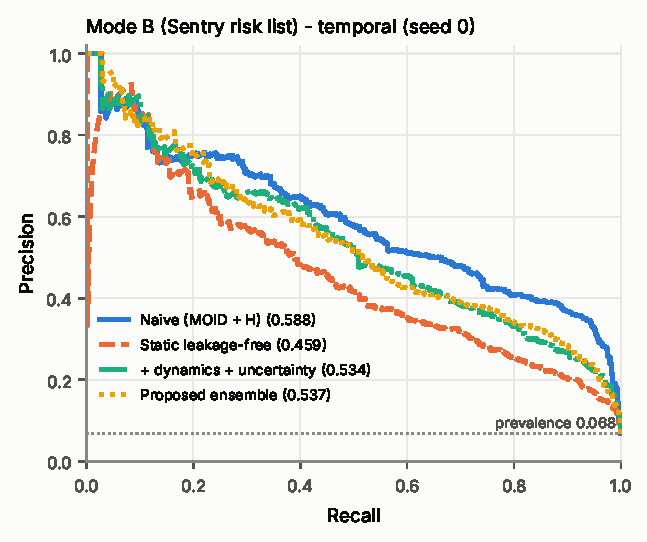
\includegraphics[width=\columnwidth]{figures/pr_sentry_temporal.pdf}
\caption{Precision--recall curves on the temporal test split for the Sentry label (five seeds pooled).}
\label{fig:pr}
\end{figure}

\begin{figure}[t]
\centering
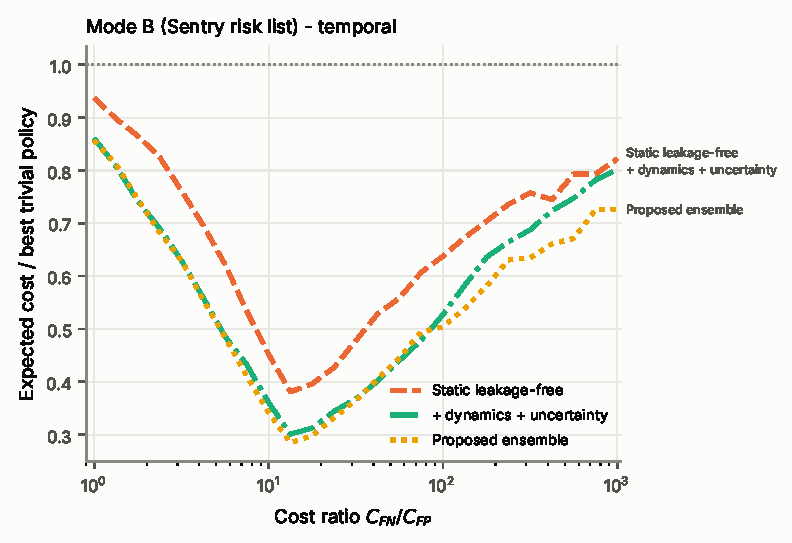
\includegraphics[width=\columnwidth]{figures/cost_sentry_temporal.pdf}
\caption{Expected cost per 1,000 objects as a function of the cost ratio $C_{\mathrm{FN}}/C_{\mathrm{FP}}$ (Sentry label, temporal split).}
\label{fig:cost}
\end{figure}

\subsection{Short observation arcs}
The gains are largest where catalogues are least certain (Table~\ref{tab:short}). For short-arc PHAs on the temporal split, PR-AUC rises from \PRPhaTemporalShortStatic{} to \PRPhaTemporalShortFull{} (\DPhaTemporalShortFull). The PHA short-arc test sets contain few positives, so the intervals are wide.

\begin{table*}[t]
\caption{Short-arc stratum (data arc $<30$~d): test size (positives) averaged over seeds, PR-AUC of the reference and of the full model, and the paired change.}
\label{tab:short}
\centering
\begin{tabular}{lcccc}
\toprule
Setting (short arcs, $<$30\,d) & $n_{\mathrm{test}}$ & Reference PR-AUC & Full PR-AUC & $\Delta$PR-AUC [95\% CI]\\
\midrule
Sentry, stratified & 3,689 (308) & 0.464 & 0.597 & +0.133 [+0.112, +0.155]\\
Sentry, temporal & 4,941 (393) & 0.415 & 0.531 & +0.117 [+0.094, +0.134]\\
PHA, stratified & 3,689 (25) & 0.255 & 0.346 & +0.091 [+0.042, +0.147]\\
PHA, temporal & 4,941 (22) & 0.188 & 0.310 & +0.121 [+0.067, +0.194]\\
\bottomrule
\end{tabular}

\end{table*}

\subsection{Loss functions and model families}
The asymmetric focal loss gives no significant difference from log-loss in any of the eight settings (Table~\ref{tab:pairwise}); with validation-based selection, plain log-loss ($\gamma=0$, $\lambda_{\mathrm{FN}}=1$) was chosen in \NFocalPlain{} of the four settings for the first seed. The ensemble is likewise indistinguishable from LightGBM in every setting, while the dual-branch MLP is significantly worse in all of them. With calibrated probabilities, moving the decision threshold achieves the intended asymmetry without changing the training objective.

\subsection{Calibration and decisions}
After Platt scaling, predicted probabilities track the observed frequencies closely above about 1\%, and are somewhat over-confident below that level (Fig.~\ref{fig:rel}). Mondrian conformal sets meet their coverage targets on average (Table~\ref{tab:conf}, Fig.~\ref{fig:conf}). For Sentry (temporal) at $\alpha_H=0.10$, the full model sends \FollowSenTempFull\% of objects to follow-up, against \FollowSenTempStatic\% for the static model at the same guaranteed hazard coverage. For the PHA temporal split, about \NCalPosPhaTemp{} positives are available for calibration, and very small $\alpha_H$ forces ``hazardous'' into most sets.

\begin{figure}[t]
\centering
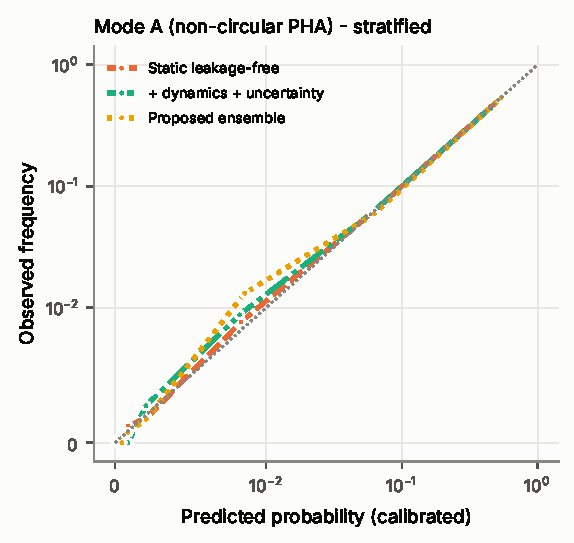
\includegraphics[width=\columnwidth]{figures/reliability_pha_stratified.pdf}
\caption{Reliability of calibrated probabilities (PHA label, stratified split).}
\label{fig:rel}
\end{figure}

\begin{figure}[t]
\centering
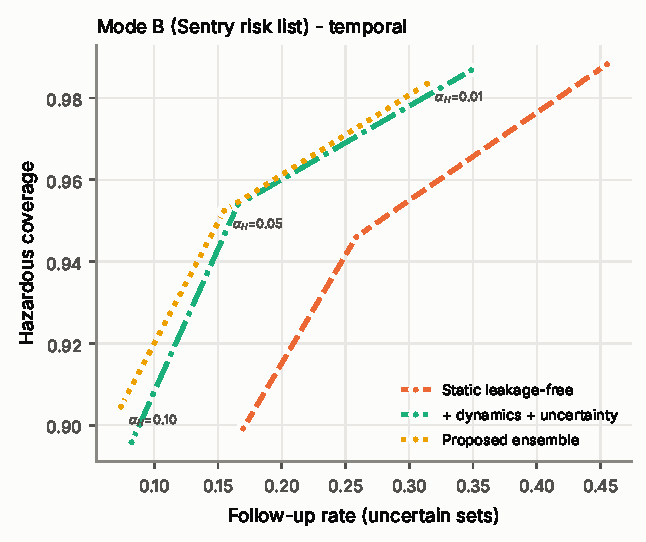
\includegraphics[width=\columnwidth]{figures/conformal_sentry_temporal.pdf}
\caption{Conformal trade-off on the Sentry temporal split: hazard coverage and follow-up rate as functions of $\alpha_H$.}
\label{fig:conf}
\end{figure}

\begin{table*}[t]
\caption{Mondrian conformal sets on the temporal splits (mean over seeds, $\alpha_B=0.10$).}
\label{tab:conf}
\centering
\begin{tabular}{llcccc}
\toprule
Target, split & Model & $\alpha_H$ & Hazard coverage & Benign coverage & Follow-up rate\\
\midrule
Sentry, temporal & Leak-free static & 0.05 & 0.946 & 0.900 & 0.258\\
 &  & 0.10 & 0.899 & 0.900 & 0.170\\
 & + dyn. + unc. & 0.05 & 0.954 & 0.900 & 0.166\\
 &  & 0.10 & 0.896 & 0.900 & 0.082\\
\midrule
PHA, temporal & Leak-free static & 0.05 & 0.936 & 0.900 & 0.019\\
 &  & 0.10 & 0.880 & 0.900 & 0.047\\
 & + dyn. + unc. & 0.05 & 0.947 & 0.900 & 0.018\\
 &  & 0.10 & 0.900 & 0.900 & 0.051\\
\bottomrule
\end{tabular}

\end{table*}

\subsection{What the model uses}
For the Sentry label, the most important input of the full model is \texttt{\TopFeatSentry} (\TopFeatSentryShare\% of total split gain), and dynamics and uncertainty features account for \DynUncShareTopFifteen\% of the gain among the 15 most important inputs. TreeSHAP contributions \cite{lundberg2020} are released for every object, from the cross-validation model that scored it. They add exactly to that model's log-odds. They also reveal a limitation: Bennu is on the Sentry list, but its listed impact window lies beyond our 50-year horizon and its clone cloud barely spreads within it, so the full model assigns it $P=\BennuPSentry\%$.

\subsection{Computational cost}
On a 4-core CPU without a GPU, the 50-year N-body propagation of all objects took \WallStageTwo~min. Propagating the clones (about 1.4 million particles) took \WallStageThree~min. Training and evaluating all models for one label and split with five seeds took \WallEvalMin--\WallEvalMax~min. Scoring an object with a trained model takes microseconds once its features exist; the clone propagation dominates the cost of features for a new object.

\section{Discussion and Limitations}\label{sec:discussion}
\emph{Emulation of Sentry.} Sentry builds its list by sampling each object's orbit uncertainty, and our clone features approximate that process. Part of the Mode B gain therefore reflects a cheap model learning to emulate Sentry rather than discovering new hazard signal. Mode A provides a label that does not come from that process, and there the clone features still add significant information beyond dynamics. A stronger test is prospective: we release a script that rescores objects later added to or removed from the Sentry list. At the time of writing, too few had changed to evaluate.

\emph{Implicit information.} The probe in Table~\ref{tab:probe} shows that ``leak-free'' means no direct access, not no information: MOID and $H$ remain largely predictable from legitimate inputs. Part of the leak-free performance on Mode A may therefore come from reconstructing the rule~\eqref{eq:pha} implicitly rather than from new physical insight.

\emph{Physics approximations.} Planetary initial conditions use approximate elements rather than DE440 \cite{park2021}. Clones sample the gravitational covariance block, so Yarkovsky and other non-gravitational effects \cite{bottke2006} are not sampled. A 50-year horizon misses risks further in the future, as the Bennu case shows. Physical priors for the X complex and for objects without taxonomy are assumptions; survey albedos such as NEOWISE \cite{mainzer2011} would reduce them.

\emph{Threats to validity.} (i) \emph{Label noise:} the PHA flag and rule~\eqref{eq:pha} disagree for \NPhaDisagree{} objects, and Sentry membership changes as observations accumulate. (ii) \emph{Selection:} only objects with a published covariance are included, so the population is not the full NEO catalogue; discovery biases \cite{granvik2018} shape both labels. (iii) \emph{Temporal drift:} the temporal split tests on later discoveries, but all labels come from one snapshot. (iv) \emph{Multiple comparisons:} we report eight settings and several variants; our conclusions rest on patterns that hold in all settings (the clone features, the MLP) or in none (the focal loss, the ensemble), not on single intervals. (v) \emph{Tuning:} minimal hyperparameter tuning may understate the neural model.

\emph{Scope.} The models score catalogued objects for triage and explanation. They are not an impact-probability estimator, and they do not replace orbit determination or impact monitoring \cite{roa2021}.

\section{Software and Data Availability}\label{sec:availability}
Code, configuration, tests, out-of-fold scores, explanations and figures are available at \url{https://github.com/vanshikhamuthanna2006-commits/neo-risk}. Every number in this paper is generated from the released results by a script. The release includes a browser-based atlas that propagates all objects on the GPU from orbital elements aligned to a common epoch by N-body integration (Fig.~\ref{fig:atlas}). It replays six close approaches from JPL Horizons trajectories, whose minimum distances agree with the JPL close-approach database to within \FlybyMaxErrKm~km on a 10-minute grid. Inputs are retrieved from public JPL services \cite{jplsbdb,jplhorizons}.

\begin{figure}[t]
\centering
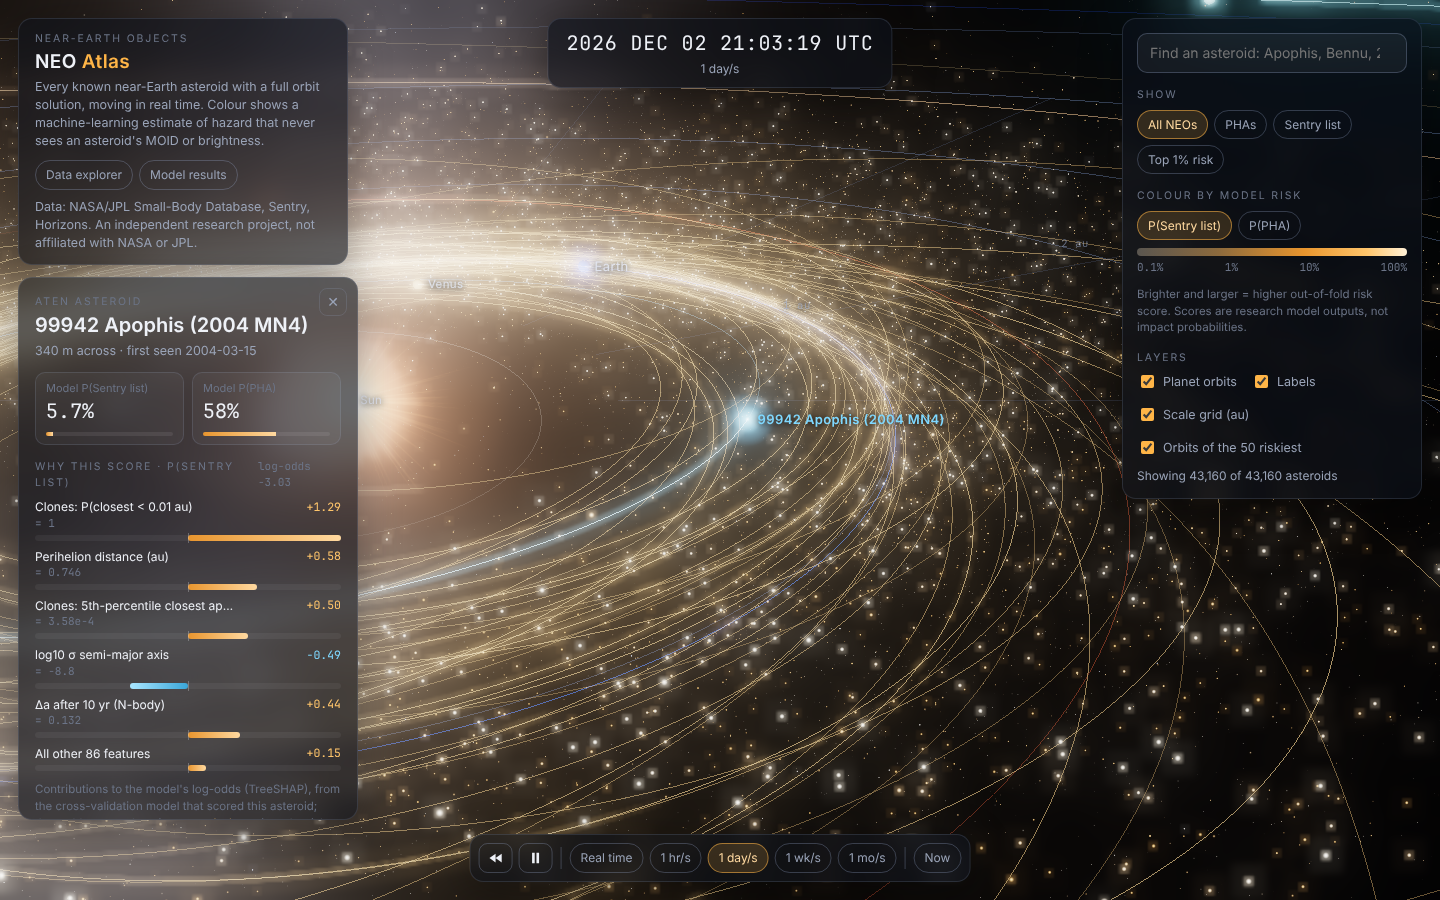
\includegraphics[width=\columnwidth]{figures/atlas.png}
\caption{The released interactive atlas: objects coloured by out-of-fold model score, the orbits of the 50 highest-scoring objects, and a per-object explanation panel.}
\label{fig:atlas}
\end{figure}

\section{Conclusion}
Removing MOID and $H$ from PHA classifiers exposes how much of their reported performance comes from the label's definition. Within a leakage-controlled protocol, features from orbit-covariance clones are the robust contribution: they improve hazard ranking beyond N-body dynamics in every setting tested, most for short-arc objects. Cost-sensitive training and model ensembling bring no measurable benefit over threshold-moving on calibrated LightGBM probabilities. Conformal sets turn the scores into follow-up decisions with stated coverage. The largest open question is prospective: whether the scores anticipate future changes to the risk lists.

\section*{Acknowledgment}
This work uses data from the NASA/JPL Small-Body Database, Sentry and Horizons services. [Funding and other acknowledgments.]

\emph{Use of AI tools (disclosure required by IEEE policy; authors to complete and confirm).} [AI system name and version] was used to write and test the analysis code, generate the figures and tables, and draft the text of all sections of this article. The authors reviewed and verified all content, checked every reference against its DOI record, and take full responsibility for the article.

\bibliographystyle{IEEEtran}
\bibliography{refs}

\end{document}
